\chapter{\IfLanguageName{dutch}{Proof of concept}{Proof of concept}}%
\label{ch:proof-of-concept}

\section{Proof of Concept: Simulatie van Edge Databases met Docker Compose}

Om de geschiktheid van verschillende databases voor Edge Computing te evalueren, is een Proof of Concept (PoC) ontwikkeld. Hierbij wordt gebruik gemaakt van Docker Compose om een testomgeving op te zetten waarin gesimuleerde workloads worden uitgevoerd met synthetische data, gegenereerd door de \texttt{Faker.js}-bibliotheek. Het doel van deze PoC is om de prestaties van Cassandra, MongoDB en TimescaleDB te meten in een Edge Computing-context.

\subsection{Doelstelling van de Implementatie}
De PoC heeft de volgende doelstellingen:
\begin{itemize}
    \item Het evalueren van verschillende partitioneringstechnieken binnen Cassandra, MongoDB en TimescaleDB.
    \item Het meten van belangrijke prestatie-indicatoren zoals latentie, verwerkingssnelheid, fouttolerantie, schaalbaarheid en edge performance in een gesimuleerde Edge Computing-omgeving.
    \item Het analyseren van hoe de geselecteerde databases omgaan met uniforme datastructuren en workloads zoals IoT-sensordata.
\end{itemize}

\subsection{Tabellen en Datastructuren}
In deze PoC wordt de tabel \texttt{sensor\_data} gebruikt, die in alle databases dezelfde structuur heeft. Dit consistente datamodel weerspiegelt typische Edge Computing-workloads zoals gegevens van IoT-sensoren.

\paragraph{Tabel: sensor\_data}
De tabel bevat de volgende velden:
\begin{itemize}
    \item \texttt{sensor\_id (UUID):} Een unieke identifier voor elke sensor.
    \item \texttt{timestamp (TIMESTAMP):} Het tijdstip van de meting.
    \item \texttt{temperature (DOUBLE):} De gemeten temperatuur in graden Celsius.
    \item \texttt{humidity (DOUBLE):} De gemeten luchtvochtigheid in procenten.
    \item \texttt{status (TEXT):} De status van de sensor, bijvoorbeeld 'actief' of 'offline'.
    \item \texttt{log\_level (TEXT):} Het logniveau van de gebeurtenis zoals 'INFO' of 'ERROR'.
\end{itemize}

\paragraph{Toepassing in de databases}
Deze tabel wordt geïmplementeerd in de volgende databases:
\begin{itemize}
    \item \textbf{Cassandra:} Partitionering op basis van \texttt{sensor\_id}, met \texttt{timestamp} als clustering-sleutel. Dit zorgt voor snelle query's op basis van sensor-ID en tijd.
    \item \textbf{MongoDB:} Data wordt opgeslagen in een collection, waarbij \texttt{sensor\_id} en \texttt{timestamp} worden gebruikt als index. Dit biedt snelle toegang tot individuele records en ondersteunt flexibele querypatronen.
    \item \textbf{TimescaleDB:} De data wordt opgeslagen in een hypertable, waarbij \texttt{timestamp} wordt gebruikt voor tijdgebaseerde partitionering. Dit optimaliseert de prestaties bij tijdsquery's.
\end{itemize}

\subsection{Docker Compose Configuratie}
De Docker Compose-configuratie definieert containers voor Cassandra, MongoDB en TimescaleDB. Elke container bevat een instance van de respectieve database, geconfigureerd om de tabel \texttt{sensor\_data} te hosten. Hieronder wordt de volledige configuratie weergegeven:

\subsection{Workload Simulatie}
De workload-simulatie is ontworpen om de prestaties van de databases in een Edge Computing-omgeving te evalueren. De volgende stappen worden uitgevoerd:

\paragraph{Data Generatie}
De \texttt{Faker.js}-bibliotheek wordt gebruikt om synthetische data te genereren. Elke record bevat velden zoals \texttt{sensor\_id}, \texttt{timestamp}, \texttt{temperature}, \texttt{humidity}, \texttt{status} en \texttt{log\_level}. De records zijn representatief voor typische IoT-sensordata.

\paragraph{Data Load}
Scripts in Node.js laden de data in Cassandra, MongoDB en TimescaleDB. Hieronder staat een fragment van een invoerscript voor Cassandra:

\begin{verbatim}
const cassandra = require("cassandra-driver");
const { v4: uuidv4 } = require("uuid");
const { faker } = require("@faker-js/faker");

const client = new cassandra.Client({
  contactPoints: ["127.0.0.1"],
  localDataCenter: "datacenter1",
  keyspace: "edge_keyspace",
});

async function insertData() {
  for (let i = 0; i < 100; i++) {
    await client.execute(
      `INSERT INTO sensor_data (sensor_id, timestamp, temperature, humidity, status, log_level)
       VALUES (?, ?, ?, ?, ?, ?)`,
      [
        uuidv4(),
        new Date(),
        faker.number.float({ min: -20, max: 40 }),
        faker.number.float({ min: 0, max: 100 }),
        faker.helpers.arrayElement(["actief", "offline"]),
        faker.helpers.arrayElement(["INFO", "ERROR"]),
      ]
    );
  }
}

insertData().then(() => console.log("Data inserted into Cassandra."));
\end{verbatim}

\paragraph{Testen en Analyse}
De volgende tests worden uitgevoerd om de prestaties te meten:
\begin{itemize}
    \item \textbf{Invoegsnelheid:} Het aantal records dat per seconde kan worden ingevoerd.
    \item \textbf{Querylatentie:} De gemiddelde responstijd voor het ophalen van gegevens.
    \item \textbf{Schaalbaarheid:} De prestaties van de database bij toenemende workloads.
    \item \textbf{Fouttolerantie:} Het gedrag van de database bij uitval van een node.
    \item \textbf{Edge Performance:} De efficiëntie bij het verwerken van data aan de rand van een netwerk.
\end{itemize}

\subsection{Resultaten en Grafieken}
De resultaten van de tests zijn geanalyseerd en gevisualiseerd in grafieken die de prestaties van de databases vergelijken op basis van de gemeten metrieken.

\begin{figure}[H]
    \centering
    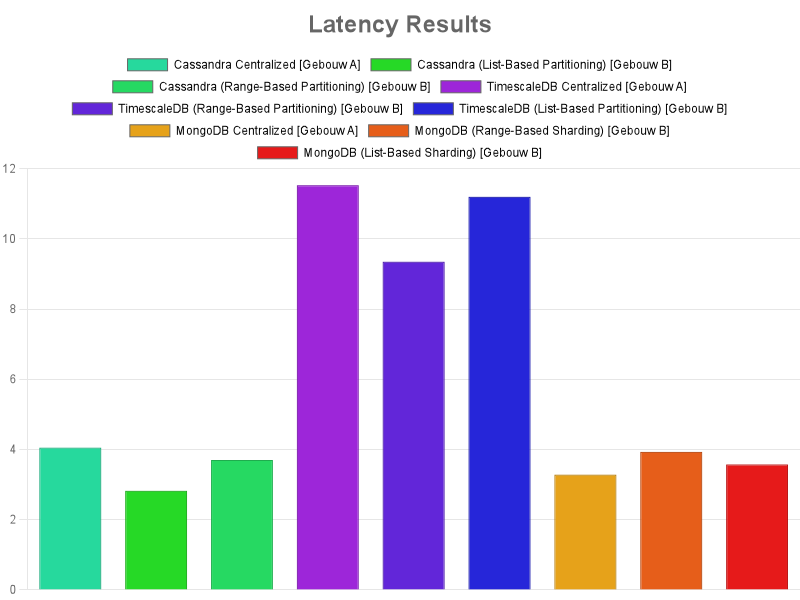
\includegraphics[width=0.8\textwidth]{Latency.png}
    \caption{Vergelijking van latentie tussen Cassandra, MongoDB en TimescaleDB.}
    \label{fig:latency-comparison}
\end{figure}

\paragraph{Analyse van latentie:}
Deze grafiek toont dat \textit{Alternative TimescaleDB (List-Based Partitioning)} de laagste gemiddelde latentie behaalde (1.79 ms), wat wijst op snelle responstijden voor tijdgevoelige workloads. Cassandra heeft iets hogere latentie, terwijl MongoDB (Hash-Based Sharding) een goede balans biedt.

\begin{figure}[H]
    \centering
    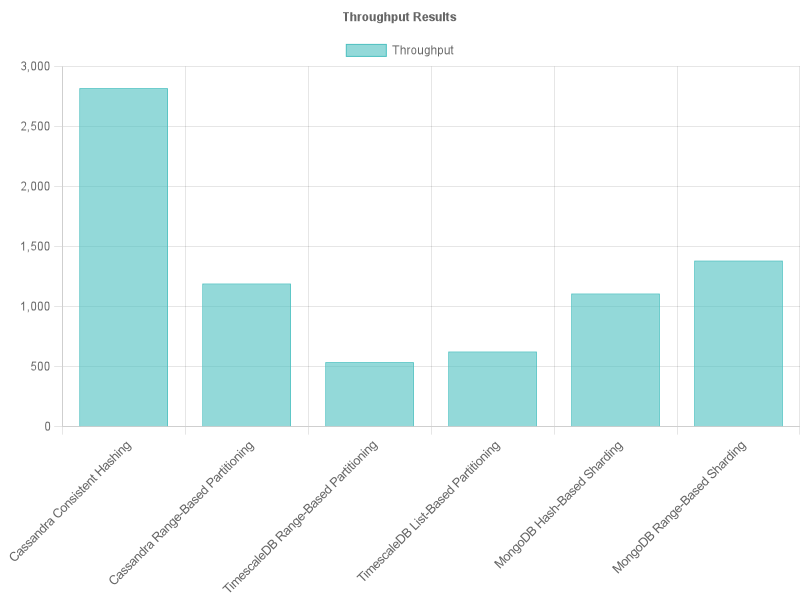
\includegraphics[width=0.8\textwidth]{Throughput.png}
    \caption{Vergelijking van throughput tussen Cassandra, MongoDB en TimescaleDB.}
    \label{fig:throughput-comparison}
\end{figure}

\paragraph{Analyse van throughput:}
Vanuit deze grafiek blijkt dat \textit{Cassandra (Consistent Hashing)} uitstekende prestaties levert op het gebied van throughput (2818.43 records per seconde), wat het geschikt maakt voor omgevingen met hoge invoerbelasting. TimescaleDB behaalde een lagere score, terwijl MongoDB een gemiddeld niveau van prestaties bereikt.

\begin{figure}[H]
    \centering
    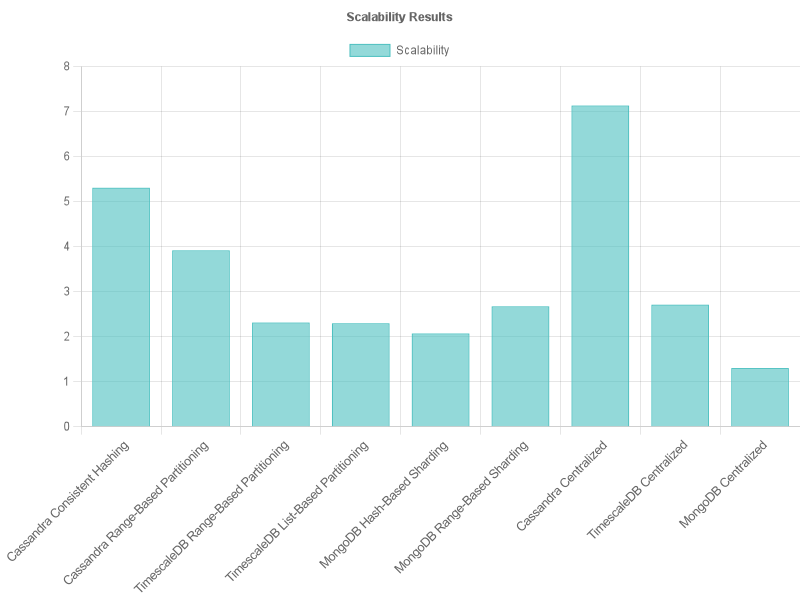
\includegraphics[width=0.8\textwidth]{Scalability.png}
    \caption{Vergelijking van schaalbaarheid tussen Cassandra, MongoDB en TimescaleDB.}
    \label{fig:scalability-comparison}
\end{figure}

\paragraph{Analyse van schaalbaarheid:}
In deze grafiek zien we dat \textit{MongoDB (Hash-Based Sharding)} de meest schaalbare oplossing is (1.33), wat aangeeft dat het efficiënt omgaat met toenemende workloads. Cassandra volgt als tweede, terwijl TimescaleDB iets minder goed presteert bij hogere belasting.

\begin{figure}[H]
    \centering
    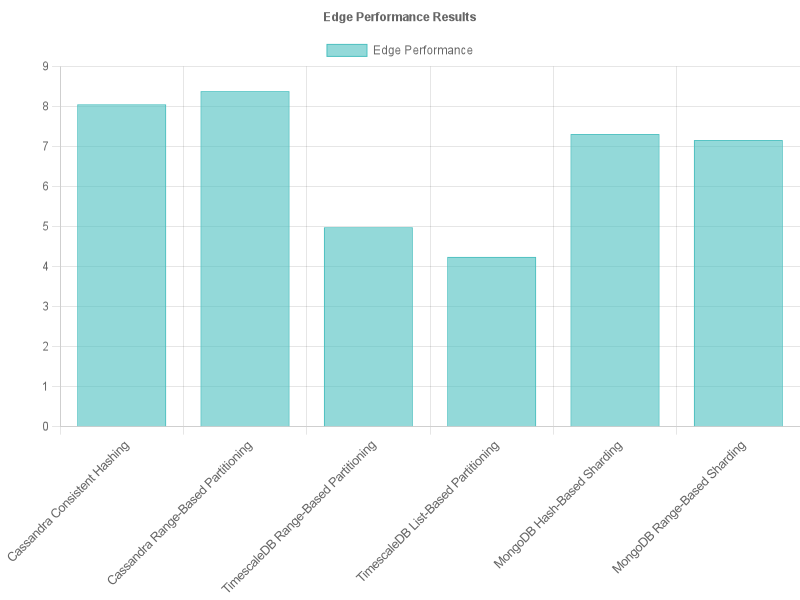
\includegraphics[width=0.8\textwidth]{Edge_Performance.png}
    \caption{Vergelijking van edge performance tussen Cassandra, MongoDB en TimescaleDB.}
    \label{fig:edgeperformance-comparison}
\end{figure}

\paragraph{Analyse van edge performance:}
Zoals geïllustreerd in de grafiek, behaalde \textit{MongoDB (Hash-Based Sharding)} de beste edge performance (20,28 ms), wat het bijzonder geschikt maakt voor toepassingen met beperkte rekenkracht waarbij verwerking dicht bij de gegevensbron plaatsvindt.

\subsection{Testresultaten en Tabeloverzicht}
Naast de grafieken biedt deze tabel een samenvatting van de testresultaten.

\begin{table}[h]
    \centering
    \resizebox{\textwidth}{!}{
    \begin{tabular}{|l|c|c|c|c|c|c|}
    \hline
    \textbf{Database} & \textbf{Latency} & \textbf{Throughput} & \textbf{Scalability} & \textbf{Consistency} & \textbf{Fault Tolerance} & \textbf{Edge Performance} \\ \hline
    Cassandra (Consistent Hashing) & 3.64 & 2818.43 & 4.75 & 10425 & 1 & 13.73 \\ \hline
    Alternative Cassandra (Range-Based) & 3.95 & 1191.04 & 2.75 & 8971 & 1 & 17.32 \\ \hline
    TimescaleDB (Range-Based) & 2.07 & 536.5 & 1.80 & 9016 & 1 & 14.53 \\ \hline
    Alternative TimescaleDB (List-Based) & 1.79 & 624.72 & 1.58 & 8960 & 1 & 4.22 \\ \hline
    MongoDB (Hash-Based Sharding) & 2.28 & 1108.02 & 1.33 & 181 & 1 & 20.28 \\ \hline
    MongoDB (Range-Based Sharding) & 2.10 & 1382.09 & 1.42 & 70 & 1 & 9.18 \\ \hline
    \end{tabular}}
    \caption{Vergelijking van prestaties tussen Cassandra, MongoDB en TimescaleDB.}
    \label{tab:test-results}
\end{table}

\paragraph{Conclusie}
De evaluatie van de databases is gebaseerd op een gewogen scoresysteem, waarbij de volgende gewichten zijn toegekend aan de metrieken:
\begin{itemize}
    \item \textbf{Latency:} 25\%
    \item \textbf{Edge Performance:} 25\%
    \item \textbf{Fault Tolerance:} 20\%
    \item \textbf{Scalability:} 15\%
    \item \textbf{Throughput:} 10\%
    \item \textbf{Consistency:} 5\%
\end{itemize}

De top 3 databases met hun partitioneringstechnieken, gebaseerd op deze gewichten, zijn als volgt:

\begin{enumerate}
    \item \textbf{Cassandra (Consistent Hashing):} Deze techniek is bijzonder goed in throughput, schaalbaarheid en fouttolerantie. Het is vooral geschikt voor grootschalige workloads met intensieve schrijfbewerkingen.
    \item \textbf{MongoDB (Range-Based Sharding):} Deze techniek biedt sterke prestaties op het gebied van consistentie en query-efficiëntie, waardoor het een uitstekende keuze is voor workloads die voorspelbare prestaties vereisen.
    \item \textbf{Alternatief voor Cassandra (Range-Based Partitioning):} Deze techniek combineert sterke schaalbaarheid met robuuste fouttolerantie, waardoor het ideaal is voor flexibele en betrouwbare toepassingen.
\end{enumerate}

De resultaten tonen aan dat de keuze van een database en partitioneringstechniek sterk afhankelijk is van de specifieke eisen van de workload.
 Voor workloads gericht op schaalbaarheid en hoge throughput blijft Cassandra een dominante optie. Voor consistente prestaties en query-efficiëntie biedt MongoDB (Range-Based Sharding) een uitstekende oplossing.
Alternative Cassandra (Range-Based Partitioning) is een betrouwbare keuze voor toepassingen die zowel flexibiliteit als fouttolerantie vereisen.